\documentclass[tikz,border=4pt]{standalone}
\usepackage[T1]{fontenc}
\usepackage[utf8]{inputenc}
\usepackage{tikz}
\usetikzlibrary{arrows.meta,positioning}

\definecolor{calyrbg}{RGB}{14,18,24}
\definecolor{calyrpanel}{RGB}{24,30,39}
\definecolor{calyrink}{RGB}{235,239,244}
\definecolor{calyrmuted}{RGB}{150,161,173}
\definecolor{calyraccent}{RGB}{92,203,255}
\definecolor{calyrline}{RGB}{45,57,72}
\definecolor{MagentaAI}{RGB}{214,116,255}

\begin{document}
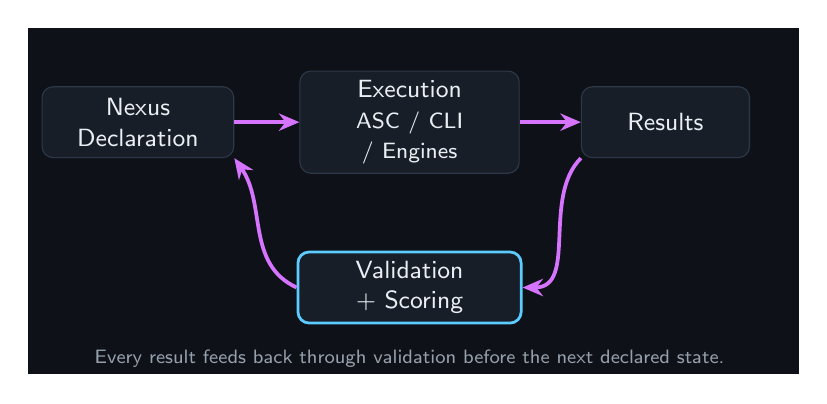
\begin{tikzpicture}[
  font=\sffamily\small,
  boxstyle/.style={draw, rounded corners=4pt, align=center,
                   fill=calyrpanel, text=calyrink, draw=calyrline,
                   minimum height=0.9cm},
  arrow/.style={-{Stealth[length=2.6mm,width=2.2mm]}, line width=1.35pt, color=MagentaAI}
]
\fill[calyrbg] (-1.4,-3.2) rectangle (8.4,1.2);
\node[boxstyle, text width=2.2cm] (nexus)      at (0,0)   {Nexus\\Declaration};
\node[boxstyle, text width=2.55cm] (exec)      at (3.45,0) {Execution\\{\footnotesize ASC / CLI / Engines}};
\node[boxstyle, text width=1.9cm] (results)    at (6.7,0) {Results};
\node[boxstyle, text width=2.6cm, draw=calyraccent, line width=1pt] (validation) at (3.45,-2.1) {Validation\\+ Scoring};
\draw[arrow] (nexus.east) -- (exec.west);
\draw[arrow] (exec.east) -- (results.west);
\draw[arrow] (results.south west) to[out=225,in=0] (validation.east);
\draw[arrow] (validation.west) to[out=155,in=305] (nexus.south east);
\node[text=calyrmuted, font=\sffamily\scriptsize, align=center] at (3.45,-3.0) {Every result feeds back through validation before the next declared state.};
\end{tikzpicture}
\end{document}
